\section{Analyse des résultats}
La figure \ref{fig:ResultatsChampsSigma} donnent une illustration des champs des contraintes pour différentes discrétisations. La table \ref{table:objectif} reprend différentes valeurs de l'objectif obtenues pour pour différentes discrétisations. Cette valeur croit bien avec le nombre de triangles, comme prédit par la théorie (voir section Modélisation). 

\begin{table}
\centering
\begin{tabular}{c|cccc}
\textbf{Discrétisation} & $N=4$ & $N=8$ & $N=12$ & $N=16$\\
\textbf{Valeur de l'objectif} & 1.3483 & 1.379409 & 1.3866 & 1.393687 \\
\end{tabular}
\caption{Valeur de l'objectif.}
\label{table:objectif}
\end{table} 

\begin{figure}[h!]
  \centering
  \begin{subfigure}[b]{0.32\textwidth}
  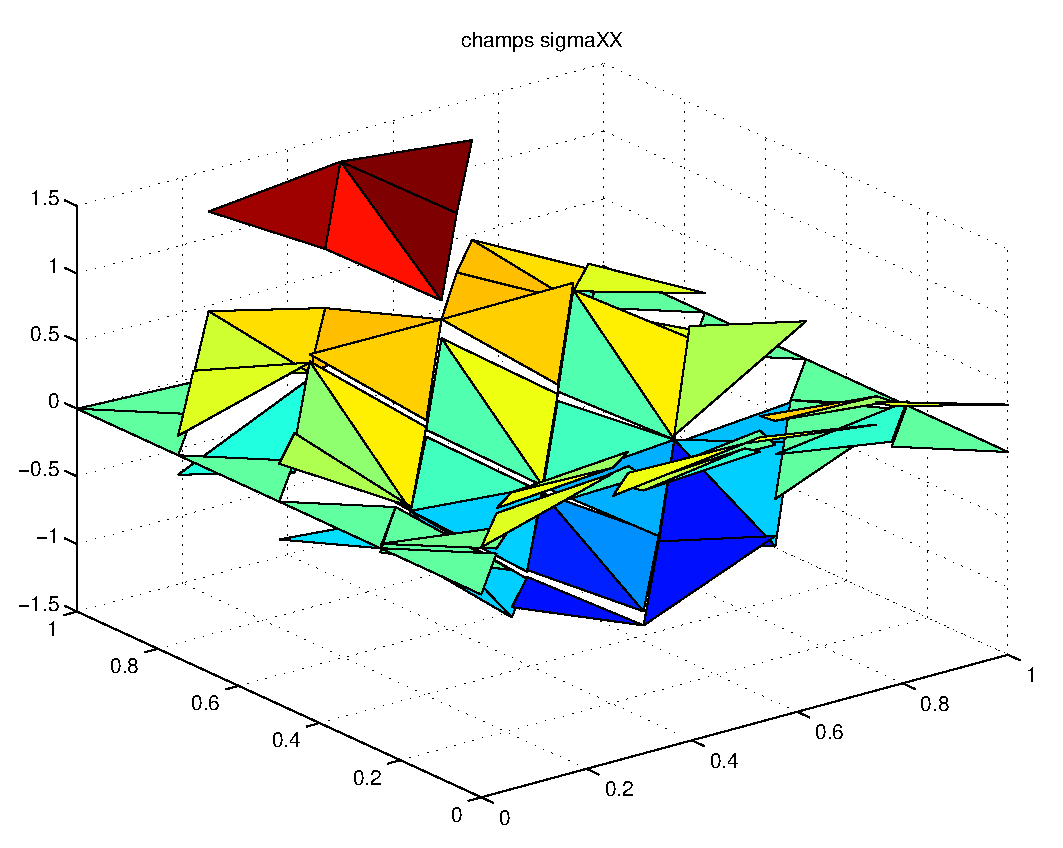
\includegraphics[width=\textwidth]{images/sigmaxxN4.eps}
  \caption{Champs $\sigma_{xx}$ pour $N=4$}
  \end{subfigure}%
  ~
  \begin{subfigure}[b]{0.32\textwidth}
  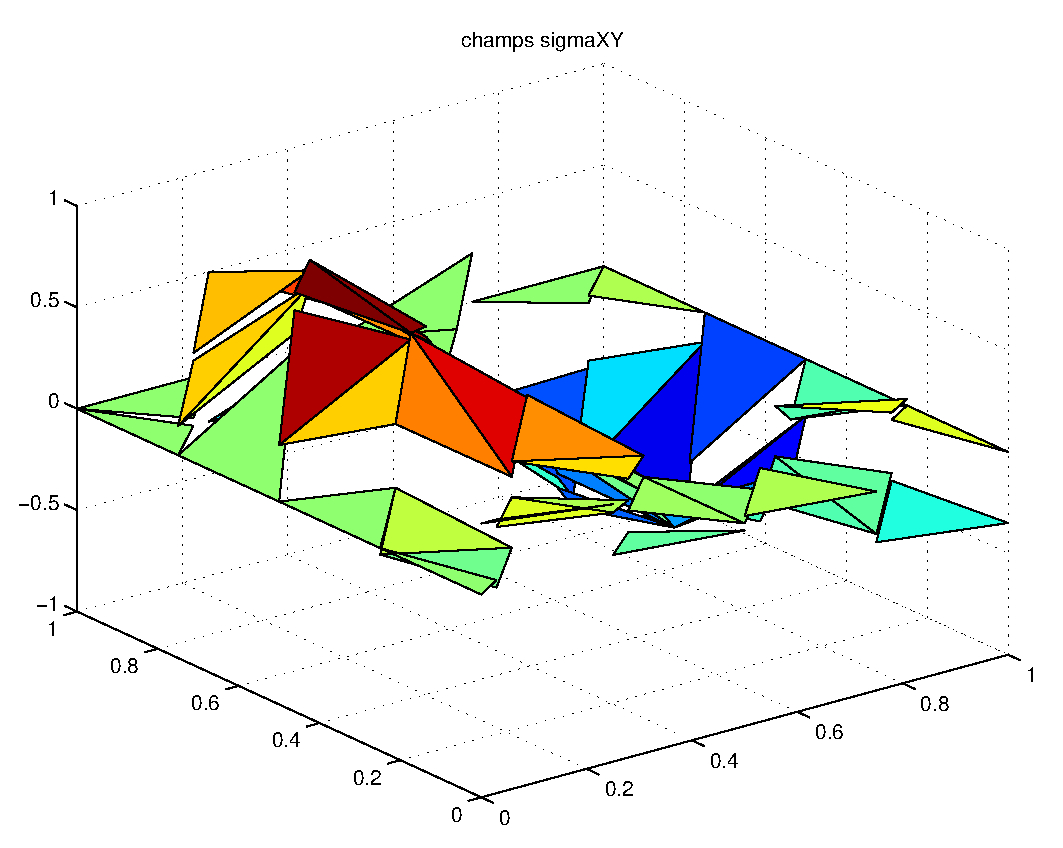
\includegraphics[width=\textwidth]{images/sigmaxyN4.eps}
  \caption{Champs $\sigma_{xy}$ pour $N=4$}
  \end{subfigure}
  ~
  \begin{subfigure}[b]{0.32\textwidth}
  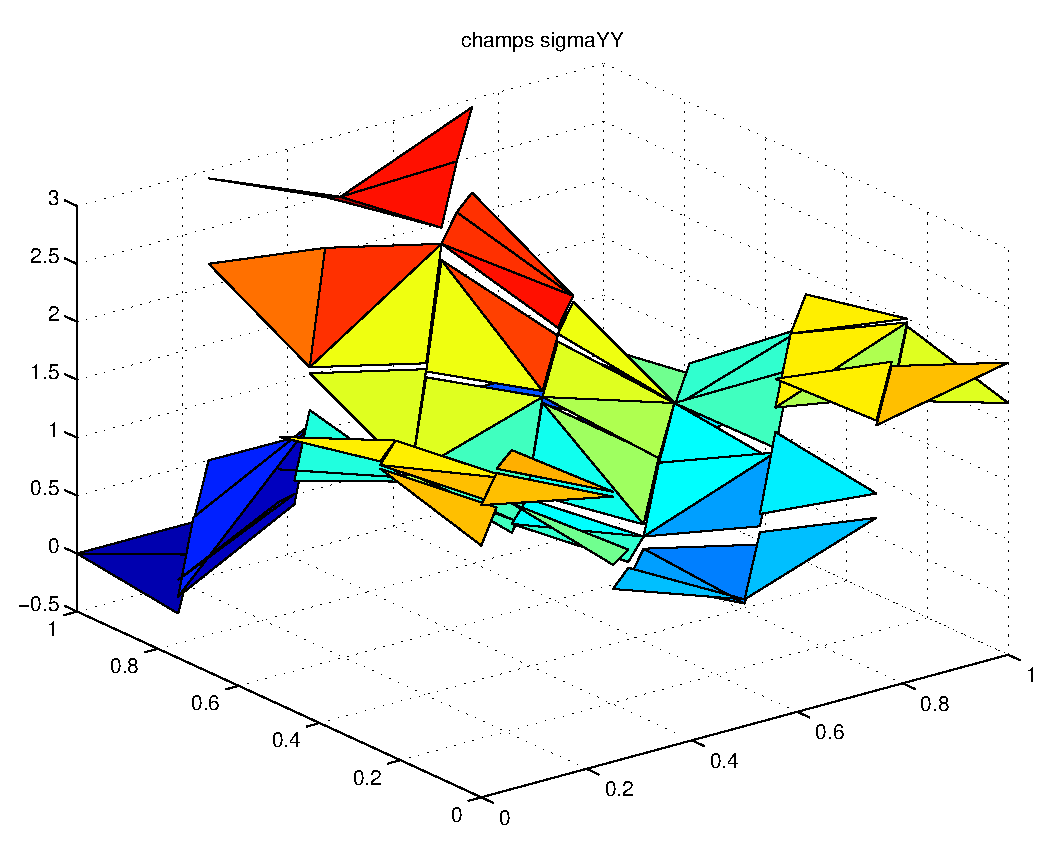
\includegraphics[width=\textwidth]{images/sigmayyN4.eps}
  \caption{Champs $\sigma_{yy}$ pour $N=4$}
  \end{subfigure}
  \begin{subfigure}[b]{0.32\textwidth}
  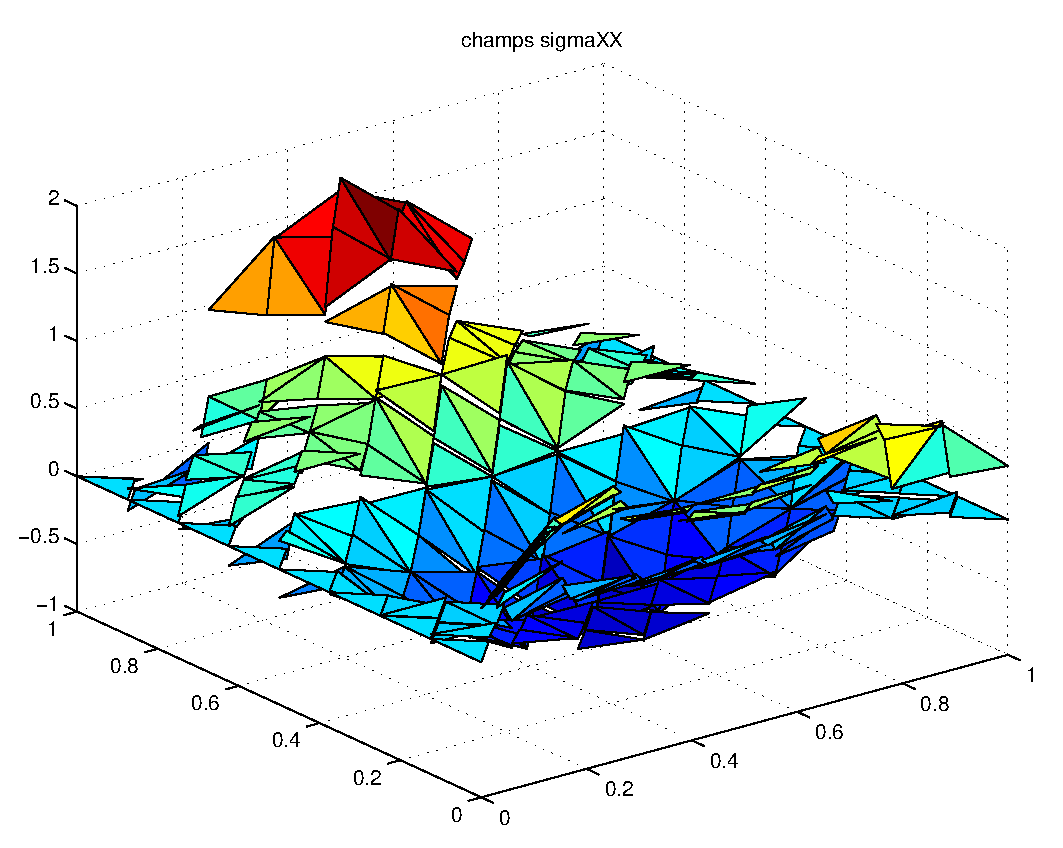
\includegraphics[width=\textwidth]{images/sigmaxxN8.eps}
  \caption{Champs $\sigma_{xx}$ pour $N=8$}
  \end{subfigure}
  ~
  \begin{subfigure}[b]{0.32\textwidth}
  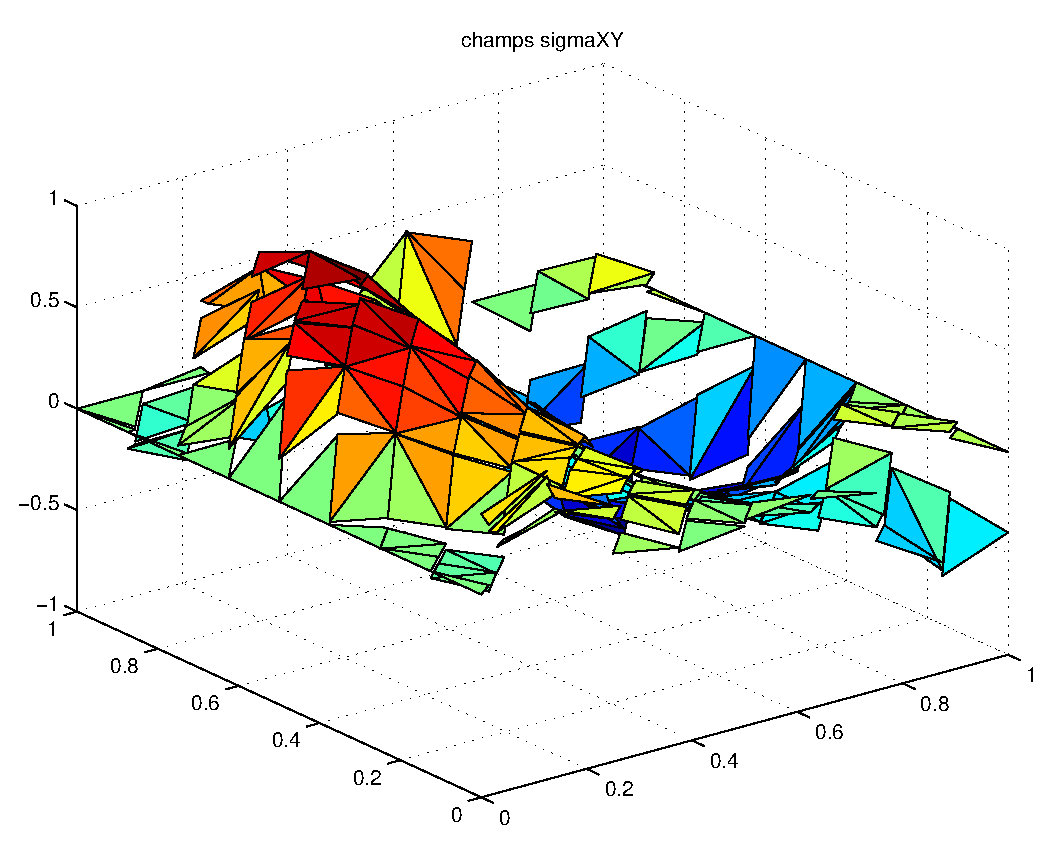
\includegraphics[width=\textwidth]{images/sigmaxyN8.eps}
  \caption{Champs $\sigma_{xy}$ pour $N=8$}
  \end{subfigure}
  ~
  \begin{subfigure}[b]{0.32\textwidth}
  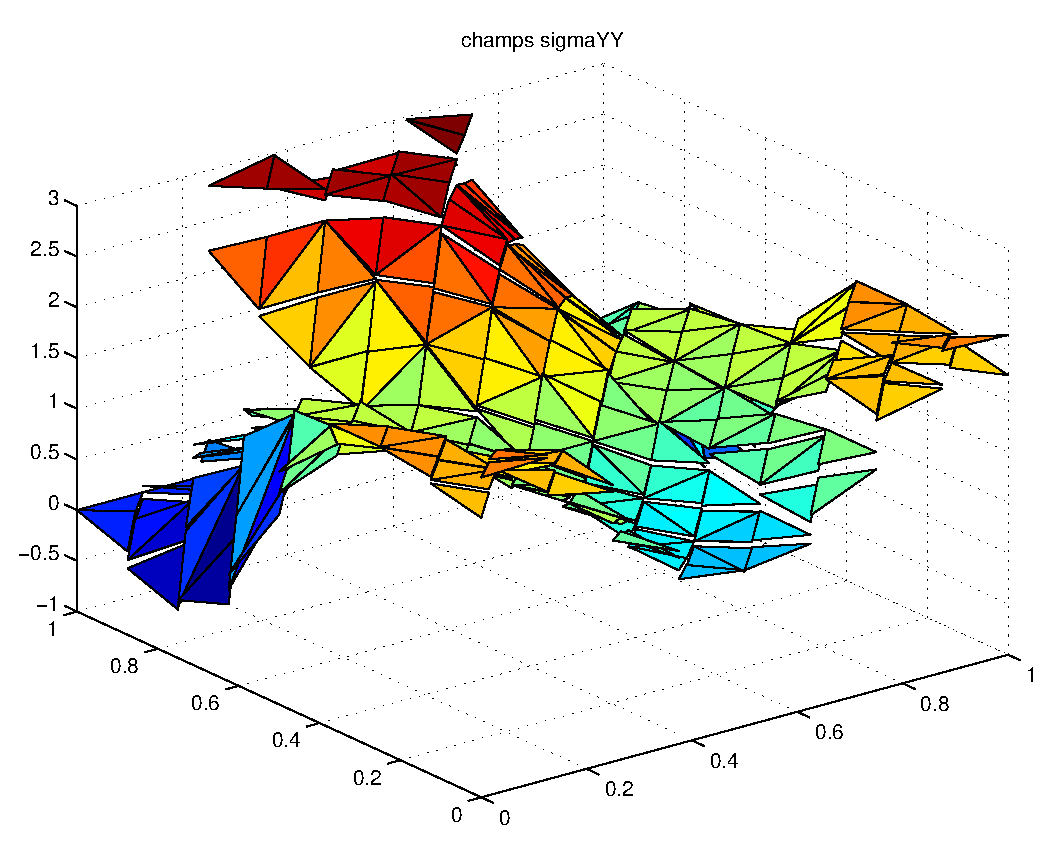
\includegraphics[width=\textwidth]{images/sigmayyN8.eps}
  \caption{Champs $\sigma_{yy}$ pour $N=8$}
  \end{subfigure}
  \begin{subfigure}[b]{0.32\textwidth}
  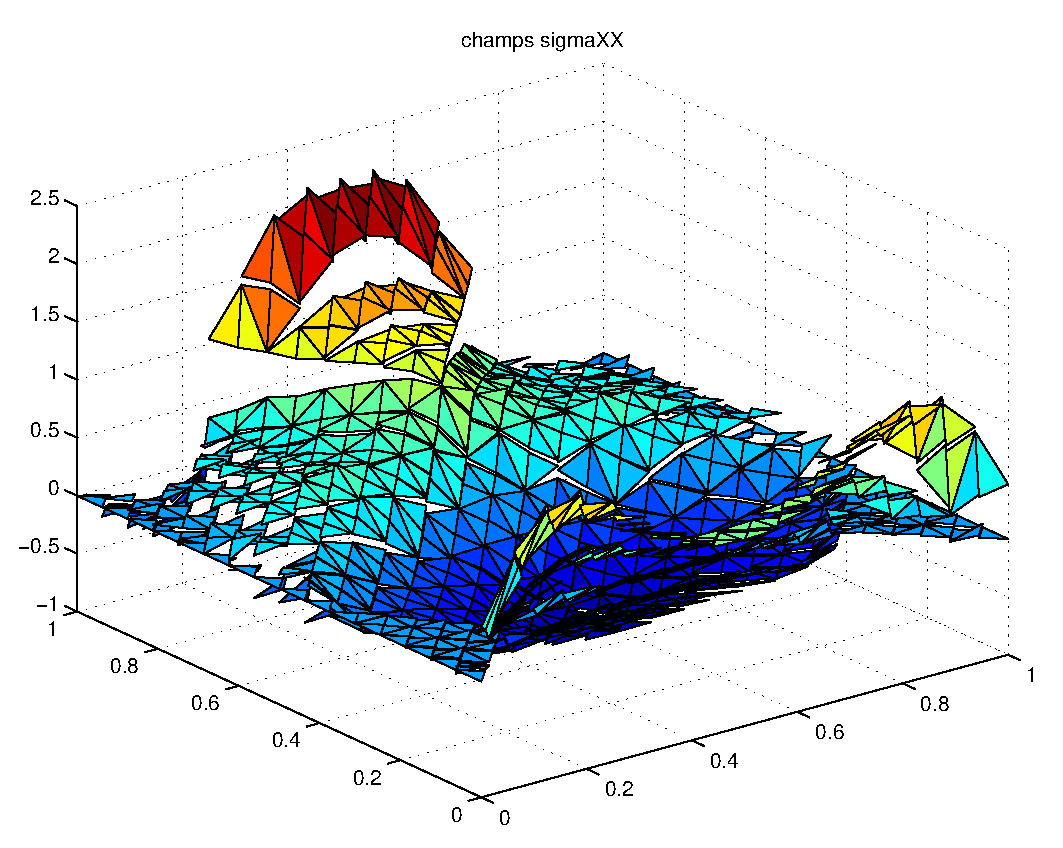
\includegraphics[width=\textwidth]{images/sigmaxxN32.eps}
  \caption{Champs $\sigma_{xx}$ pour $N=16$}
  \end{subfigure}
  ~
  \begin{subfigure}[b]{0.32\textwidth}
  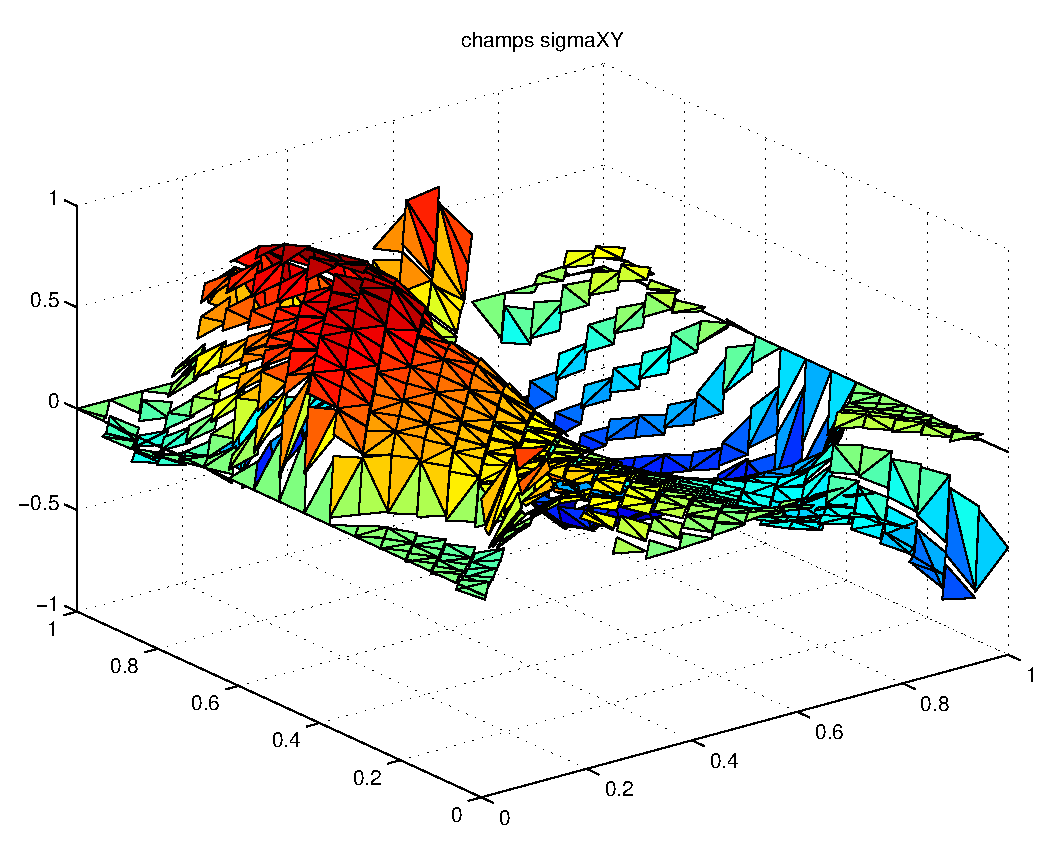
\includegraphics[width=\textwidth]{images/sigmaxyN32.eps}
  \caption{Champs $\sigma_{xy}$ pour $N=16$}
  \end{subfigure}
  ~
  \begin{subfigure}[b]{0.32\textwidth}
  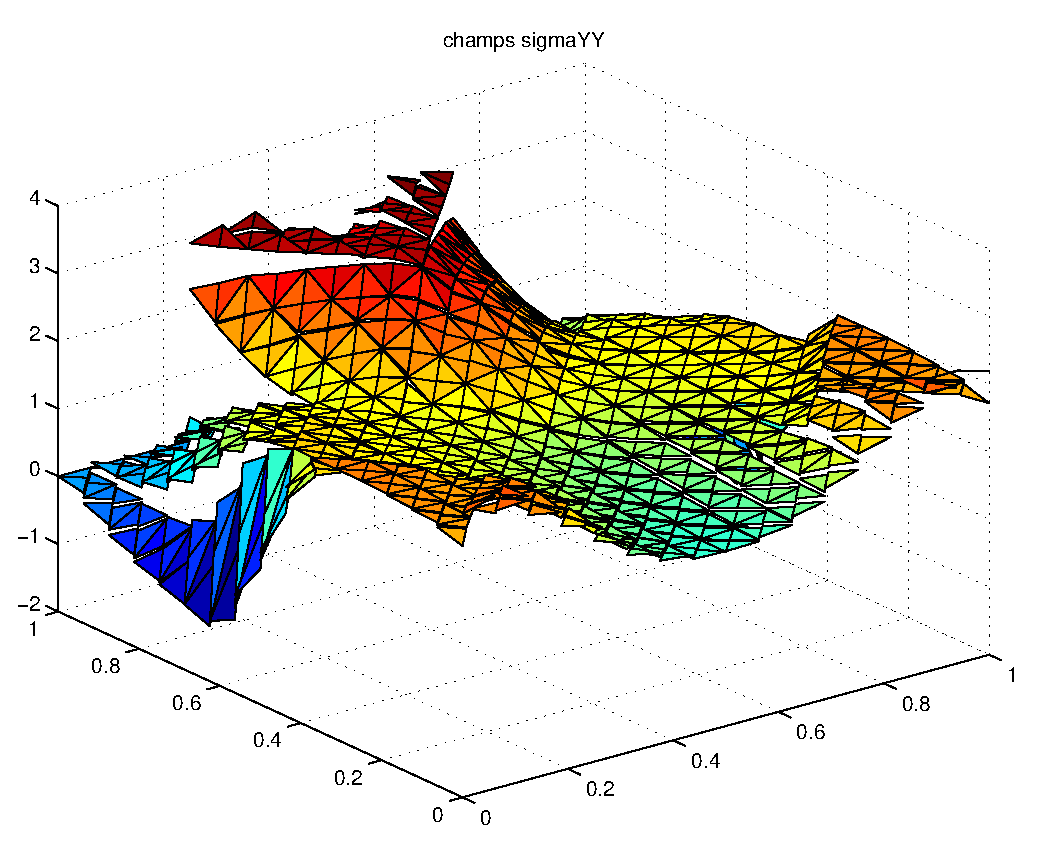
\includegraphics[width=\textwidth]{images/sigmayyN32.eps}
  \caption{Champs $\sigma_{yy}$ pour $N=16$}
  \end{subfigure}
  \caption{}
  \label{fig:ResultatsChampsSigma}
  
 

  
\end{figure}

\subsection{Complexité et performances}
Rappelons que la complexité de pire cas d'une méthode à pas longs  $\mathcal{O}(\nu log(\frac{1}{\epsilon})$. Bien que cette complexité de pire cas soit supérieure à la complexité de pire cas d'une méthode à pas courts, donnée par $\mathcal{O}(\sqrt{\nu} \log(\frac{1}{\epsilon}))$. Nous ne pouvons cependant pas nous fier à cette borne car les résultats de la méthode à pas long sont en pratique bien meilleur.


Nous tentons donc d'améliorer notre méthode, apparemment sans succès (v. figure \ref{fig:speedimp}).\\
Nous avons introduit deux améliorations sous la forme d'heuristiques : 
\begin{itemize}
\item Recherche en ligne : au lieu de proposer un pas de Newton multiplié par $\frac{1}{1+\delta}$ lorsque $\delta>1$, on essaie de trouver la longueur de pas maximale telle que l'itéré reste admissible

\item $\sigma$ adaptatif : Cette heuristique adapte simplement la valeur de $\sigma$. Intuitivement, si l'on utilise un $\sigma$ plus petit le nombre de pas de Newton nécessaire par étape sera diminué. On diminue donc $\sigma$ quand le nombre de pas de Newton à l'étape précédente sera trop important, et on le diminuera quand il sera petit.

\end{itemize}
\begin{figure}[!h]
\centering
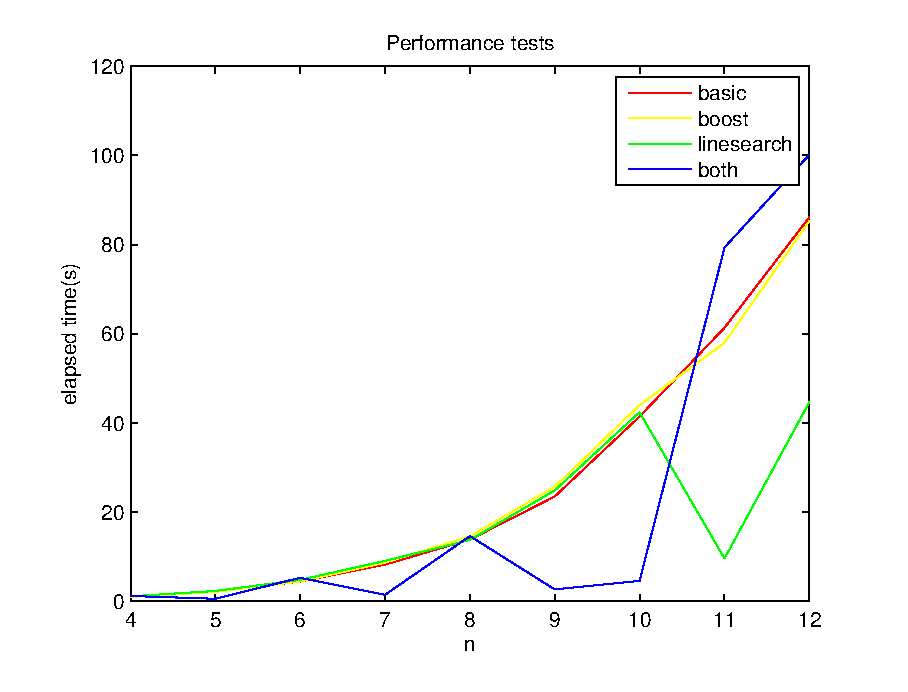
\includegraphics[width=6cm]{images/speedimp.eps}
\caption{Evolution des temps de calcul pour la méthode et ses "améliorations"\label{fig:speedimp}}
\end{figure}

